The custom instructions are implemented and validated with Verilator v4.032 using the SweRV-EL2 v1.3 core.

The first step is adding the logic in the decoding stage to recognize the opcode of the custom instructions. 
Espresso logic minimizer \cite{250190} is used in this stage.

Then, the corresponding logic is added in the execution stage. Since carry-less multiplication and binary 
multiplication share the same module within the core, the polynomial reduction module is also implemented 
in the same block. The block diagram of the SweRV-EL2 core is shown in Fig. \ref{fig:swerv}.

\begin{figure}[b]
    \centering
    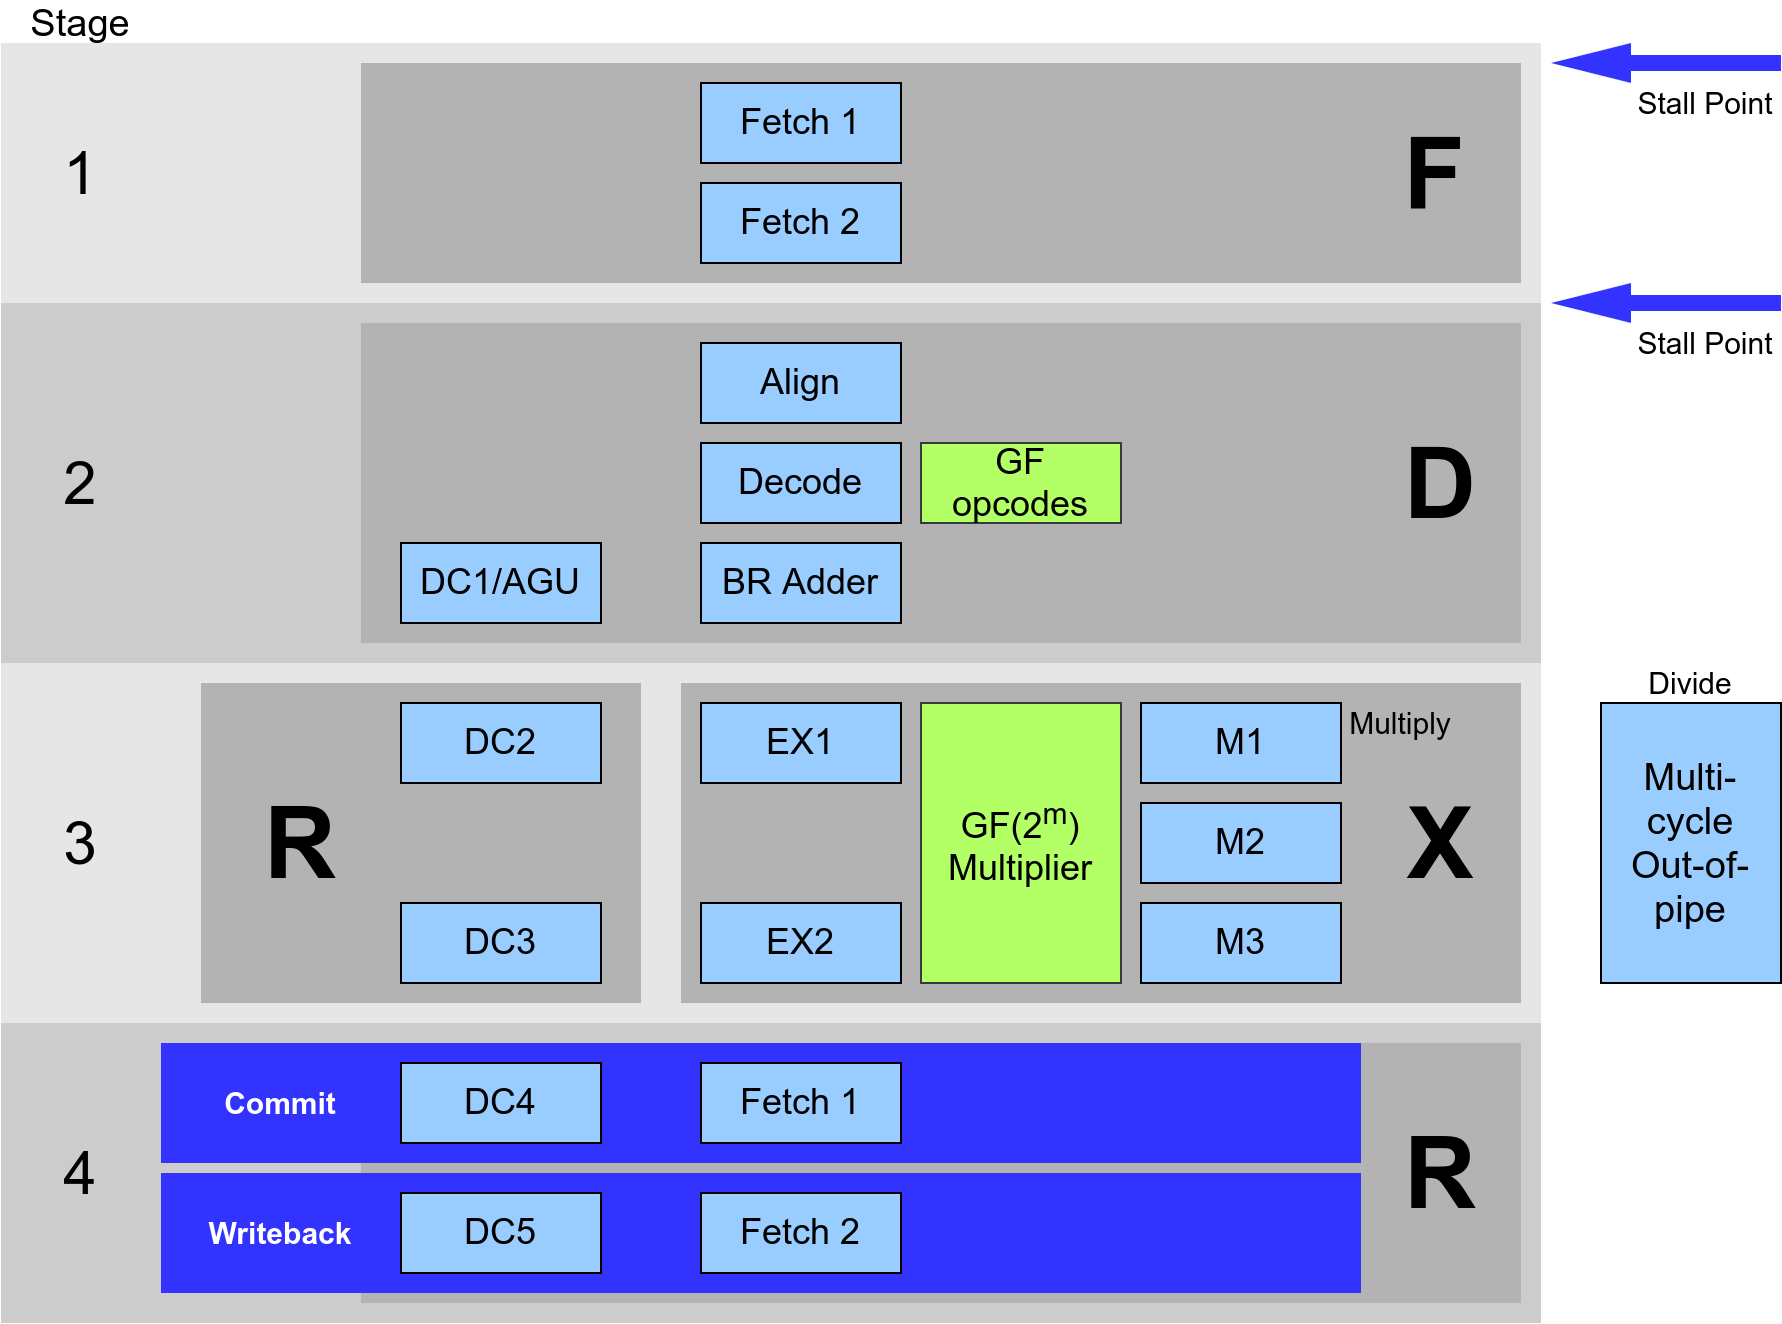
\includegraphics[width=0.95\linewidth]{img/swerv.png}
    \caption{SweRV EL2 Core Pipeline \cite{swervel2}.}
    \Description{SweRV EL2 Core Pipeline.}
    \label{fig:swerv}
\end{figure}

\begin{table*}[tp]
    \begin{tabular}{ccccccc}
    \rowcolor[HTML]{C0C0C0} 
    AES128                               & CBC Enc.             & CBC Dec.             & CTR Enc.             & CTR Dec.             & ECB Enc.             & ECB Dec.             \\ \hline
    \cellcolor[HTML]{EFEFEF}RV32IMC      & 160626               & 163584               & 161228               & 161228               & 41475                & 42082                \\
    \cellcolor[HTML]{EFEFEF}custom       & 22969                & 22759                & 23583                & 23583                & 7054                 & 6917                 \\
    \cellcolor[HTML]{EFEFEF}Reduc. \%    & 85.70                & 86.09                & 85.37                & 85.37                & 82.99                & 83.56                \\
    \multicolumn{1}{l}{}                 & \multicolumn{1}{l}{} & \multicolumn{1}{l}{} & \multicolumn{1}{l}{} & \multicolumn{1}{l}{} & \multicolumn{1}{l}{} & \multicolumn{1}{l}{} \\
    \rowcolor[HTML]{C0C0C0} 
    AES192                               & CBC Enc.             & CBC Dec.             & CTR Enc.             & CTR Dec.             & ECB Enc.             & ECB Dec.             \\ \hline
    \cellcolor[HTML]{EFEFEF}RV32IMC      & 196218               & 200144               & 196564               & 196564               & 50891                & 51836                \\
    \cellcolor[HTML]{EFEFEF}custom       & 28105                & 27775                & 28719                & 28719                & 8902                 & 8735                 \\
    \cellcolor[HTML]{EFEFEF}Reduc. \%    & 85.68                & 86.12                & 85.39                & 85.39                & 82.51                & 83.15                \\
    \multicolumn{1}{l}{}                 & \multicolumn{1}{l}{} & \multicolumn{1}{l}{} & \multicolumn{1}{l}{} & \multicolumn{1}{l}{} & \multicolumn{1}{l}{} & \multicolumn{1}{l}{} \\
    \rowcolor[HTML]{C0C0C0} 
    AES256                               & CBC Enc.             & CBC Dec.             & CTR Enc.             & CTR Dec.             & ECB Enc.             & ECB Dec.             \\ \hline
    \cellcolor[HTML]{EFEFEF}RV32IMC      & 230027               & 234713               & 230897               & 230897               & 58553                & 59568                \\
    \cellcolor[HTML]{EFEFEF}custom       & 31434                & 30984                & 32048                & 32048                & 8944                 & 8747                 \\
    \cellcolor[HTML]{EFEFEF}Reduc. \%    & 86.33                & 86.80                & 86.12                & 86.12                & 84.72                & 85.32               
    \end{tabular}
    \caption{Number of instructions required for AES (RV32IMC vs custom).}
    \label{tab:aes}
    \end{table*}

Once the logic is implemented, the binutils and gdb modules of the RISC-V toolchain are modified to recognize the new instructions (Fig. \ref{fig:instr}).
In this way, we can run tests of different algorithms using the C language and compare the efficiency between the RV32IMC base and custom instructions.
In this work, a performance evaluation for AES and Reed-Solomon codes is made.

\subsection{AES performance} 

The C code was generated for the different key sizes (AES128, AES192, and AES256) and encryption schemes (CBC, CTR, and ECB). Another version was created with the custom instructions replacing
the code segments where the GF multiplication appears. 
Then, they were compiled with the following flags: 

\begin{center}
\textbf{-O3 -fomit-frame-pointer -fPIC -no-pie}
\end{center}

\begin{table}[b]
    \begin{tabular}{ccclcc}
    \multicolumn{1}{l}{}              & \multicolumn{2}{c}{\cellcolor[HTML]{C0C0C0}RS(255,247)}         &                          & \multicolumn{2}{c}{\cellcolor[HTML]{C0C0C0}RS(255,239)}         \\
    \cellcolor[HTML]{FFFFFF}          & \cellcolor[HTML]{C0C0C0}Encode & \cellcolor[HTML]{C0C0C0}Decode & \cellcolor[HTML]{FFFFFF} & \cellcolor[HTML]{C0C0C0}Encode & \cellcolor[HTML]{C0C0C0}Decode \\ \hline
    \cellcolor[HTML]{EFEFEF}RV32IMC   & 126232                         & 124329                         &                          & 246583                         & 248598                         \\
    \cellcolor[HTML]{EFEFEF}custom    & 23775                          & 18564                          &                          & 48082                          & 37080                          \\
    \cellcolor[HTML]{EFEFEF}Reduc. \% & 81.17                          & 85.07                          &                          & 80.50                          & 85.08                         
    \end{tabular}
    \caption{Instructions required for RS codes.}
    \label{tab:rs}
\end{table}
\begin{table*}[tp]
    \begin{tabular}{ccccccccc}
    \rowcolor[HTML]{C0C0C0} 
    SweRVolf                        & Slice LUTs           & Slice Registers      & F7 Muxes             & F8 Muxes             & Slice                          & LUT as logic         & LUT as memory        & Block RAM            \\ \hline
    \cellcolor[HTML]{EFEFEF}std     & 24714                & 12969                & 459                  & 78                   & \cellcolor[HTML]{FFCE93}7115   & 24427                & 287                  & 14                   \\
    \cellcolor[HTML]{EFEFEF}custom  & 26073                & 13006                & 531                  & 84                   & \cellcolor[HTML]{FFCE93}7521   & 25786                & 287                  & 14                   \\ \hline
    \cellcolor[HTML]{EFEFEF}Inc. \% &                      &                      &                      &                      & \cellcolor[HTML]{FFCE93}5.71\% &                      &                      &                      \\
    \multicolumn{1}{l}{}            & \multicolumn{1}{l}{} & \multicolumn{1}{l}{} & \multicolumn{1}{l}{} & \multicolumn{1}{l}{} & \multicolumn{1}{l}{}           & \multicolumn{1}{l}{} & \multicolumn{1}{l}{} & \multicolumn{1}{l}{} \\
    \rowcolor[HTML]{C0C0C0} 
    SweRV-EL2                       & Slice LUTs           & Slice Registers      & F7 Muxes             & F8 Muxes             & Slice                          & LUT as logic         & LUT as memory        & Block RAM            \\ \hline
    \cellcolor[HTML]{EFEFEF}std     & 18605                & 7651                 & 341                  & 74                   & \cellcolor[HTML]{FFCE93}5329   & 18605                & 0                    & 0                    \\
    \cellcolor[HTML]{EFEFEF}custom  & 19974                & 7688                 & 413                  & 80                   & \cellcolor[HTML]{FFCE93}5699   & 19974                & 0                    & 0                    \\ \hline
    \cellcolor[HTML]{EFEFEF}Inc. \% &                      &                      &                      &                      & \cellcolor[HTML]{FFCE93}6.94\% &                      &                      &                     
    \end{tabular}
    \caption{Logic utilization for SweRVolf and SweRV-EL2, implemented on Nexys A7.}
    \label{tab:area}
\end{table*}

The \textbf{typical\_pd} and \textbf{fpga\_optimize} settings were used for the SweRV-EL2 core. These configurations create a lightweight processor to implement on the Nexys A7 FPGA.

Table \ref{tab:aes} shows the number of instructions required for the base and custom instructions for each encryption method. It can be seen that for all cases, a significant reduction of 80\% can be reached. 
For example, for AES256, the number of base instructions needed for CBC encryption is 230027 instructions, while using the instructions custom only needs 31434.

Regarding the code size reduction, it was observed that it is greater than 35\% for all cases.

\subsection{Reed-Solomon performance} 

The same was done for the Reed-Solomon code performance comparison. A program in C code has been created with the encryption and decryption routine for RS (255,247) and RS (255,239). And then, another 
version was created with the custom instructions, replacing the multiplication of finite fields.

The same SweRV-EL2 configurations as for AES were kept, and they were also compiled with the same GCC flags.

Table \ref{tab:rs} shows the number of instructions required to encrypt and decrypt the RS (255,247) and RS (255,239) codes. 
As we can see here, for example, the instructions required to encode in RS have been reduced by 81.17\% (255,247), 
being 126232 instructions for RV32IMC and 23775 for custom instructions.

\subsection{Logic utilization} 

\begin{figure}[b]
    \centering
    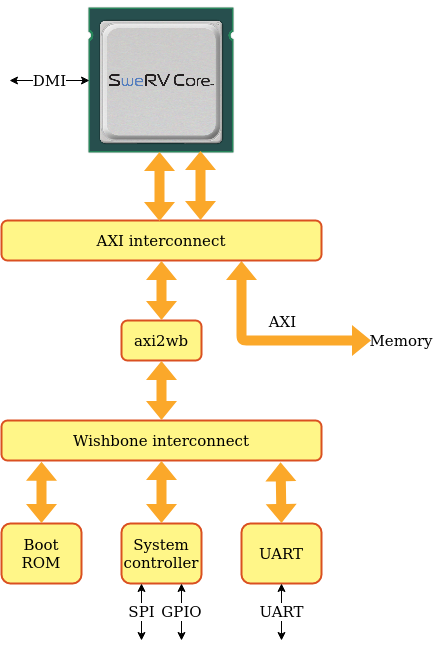
\includegraphics[width=0.7\linewidth]{img/swervolf.png}
    \caption{SweRVolf \cite{swervolf} core block diagram.}
    \Description{SweRVolf \cite{swervolf} core block diagram.}
    \label{fig:swervolf}
\end{figure}

In order to implement in an FPGA (Nexys A7), the SweRV-EL2 core was integrated into SweRVolf \cite{swervolf} SoC, 
which consists of the SweRV CPU with a boot ROM, AXI4 interconnect, UART, SPI, \mbox{RISC-V} timer and GPIO (See Fig. \ref{fig:swervolf}).

Two different SoC versions were created, one with the base instructions and the other with the custom instructions, 
both with the extension Zbc \cite{swervel2} enabled.

Table \ref{tab:area} shows the logic utilization for the standard and custom version. It can be seen that there is a 5.71\% increase in the 
number of slices at the SoC level and 6.94\% at the processor level.

Regarding the clock frequency, both work at 50 MHz. There was no decrease in frequency due to the addition of the extra logic for the
custom instructions.

